  
\pgfdeclarelayer{background}
\pgfdeclarelayer{foreground}
\pgfsetlayers{background,main,foreground}
\begin{tikzpicture}[->,>=stealth',shorten >=1pt,auto,node distance=1.3cm,
  thick,main node/.style={circle,fill=black!15,draw,font=\sffamily}]

\node[hierNode, double,label=east:300] (i) [xshift=-.2cm, yshift=-.3cm] {i}; 
\node[hierNode, cStyle, label=south:60] (c) [below of=i] {c}; 
\node[hierNode,bStyle, label=south:140] (b) [left of=c] {b}; 
\node[hierNode, dStyle, label=south:100] (d) [right of=c] {d}; 

 
  \path[every node/.style={font=\sffamily\tiny}]
   (i) edge node [right] {} (b)
   	     edge node [right] {} (c)
   	     edge node [right] {} (d)      ;   	     
  
 
\node[optboundaries, text width=8.9em, text height = 6.8em] (jOpt) at (-0.2,-1.0) {};  
 
      
\node[overlay,align=left,rectangle callout,%
      callout absolute pointer=(b.north),fill=isseorange!50] (bubble) at (-0.4,1.4) {Wie vermeide ich \\ meinen Speicher \\über 90\% zu füllen?}; 

\onslide<2->{      
\node[align=left,rectangle,dashed,rounded corners, rectangle callout, text width = 6cm, text height = 5.5cm,
      callout absolute pointer=(bubble.east),fill=black!5] at (6.5,-1.4) {}; 
};

\pgfmathsetmacro{\XOr}{5.3}
\pgfmathsetmacro{\YOr}{-1.2}
\pgfmathsetmacro{\YHeight}{2}
\pgfmathsetmacro{\XWidth}{2.5}
\pgfmathsetmacro{\YXOr}{(\YOr + \YHeight}
\pgfmathsetmacro{\XYOr}{(\XOr + \XWidth}

\coordinate (origin) at (\XOr,\YOr);
\coordinate (originX) at (\XOr,\YXOr);
\coordinate (originY) at (\XYOr,\YOr);

\onslide<3->{      

}


 \begin{pgfonlayer}{foreground}
 \tikzset{
   main node/.style={rectangle,
                     rounded corners,
   					 fill=black!15,
   					 draw,
   					 minimum width=3.5em,
   					 text centered,
                     inner sep=2.5pt,	 
   					 font=\sffamily
   					},
   treestyle/.style={rectangle,fill=black!15,draw,font=\sffamily},
   constraint/.style={circle,fill=black!15,draw,font=\sffamily\small},
   constraint_satisfied/.style = {constraint, fill=white},
   constraint_violated/.style = {constraint, fill=black!25},
}

       \tikzstyle{every state}=[circle,fill=black!25,minimum size=17pt,inner sep=.2pt]
\onslide<3->{      
\draw [black!85,fill=white] (5.0,0.5) rectangle (9.0,-1.8);
\node[main node, style={font=\sffamily\footnotesize}] (5) at (7.05,-0.2) {\gasFull};
\node[main node, style={font=\sffamily\footnotesize}] (6) [below left of=5,xshift=-1.4] {\ecoSweet};
\node[main node, style={font=\sffamily\footnotesize}] (7) [below right of=5,xshift=2.1] {\onOff};
%\node[main node, style={font=\sffamily\footnotesize},double] (hardConstraint) [below left of=7,xshift=-3.1,yshift=7] {$\mathsf{maxProd}$};

%\node[text width=2cm, anchor=west, left] at (7.2, -1.8) { \textsc{TPD} };

\path[every node/.style={font=\sffamily\tiny}]
  (6) edge node [right] {} (5)
  (7) edge node [right] {} (5)
;
}
%
%\node[overlay] at (6.5, 0.0) {
%\only<4->{      
% 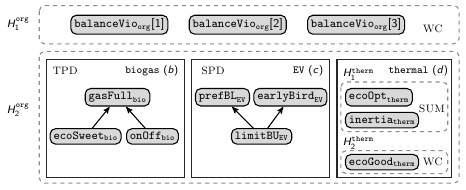
\includegraphics[width=.4\textwidth]{img/pvs.png} } };
% 
    \end{pgfonlayer}

\end{tikzpicture}
